% !TeX root = ./main.tex
\documentclass[main]{subfiles}
\begin{document}
\part{Дифференциальная геометрия кривых}
\chapter{Понятие кривой} \marginpar{05.09.22}
Кривую можно задать множеством способов, например:
\begin{itemize}
    \item в декартовых координатах: $y = f(x)$
    \item в полярных координатах: $r = r(\phi)$
    \item неявным уравнением: $F(x,y) = 0$
\end{itemize}
но обычно её задают в параметрическом виде:
\[\begin{cases}
        x = x(t) \\
        y = y(t) \\
        z = z(t)
    \end{cases}\]
В таком случае кривая
\begin{itemize}
    \item в декартовых координатах принимает вид: $\displaystyle\begin{cases}
                  x = t \\
                  y = f(t)
              \end{cases}$
    \item в полярных координатах: $\displaystyle \begin{cases}
                  x = r(t) \cos t \\
                  y = r(t) \sin t
              \end{cases}$
    \item для неявных уравнений свои методы, т.к. не очень понятно как с ними работать
\end{itemize}

Например, для неявных уравнений существует следующая теорема:
\begin{theorem*}[О неявной функции]
    Если $F(x,y) = 0$ и $F(x_0, y_0) = 0$,
    а так же $\frac{\partial F}{\partial y}\rvert_{(x_0, y_0)} \neq 0$,
    $\frac{\partial F}{\partial x}, \frac{\partial F}{\partial y}$ существуют и непрерывны в окрестности $(x_0, y_0)$,
    тогда существует $f(x)$ в некоторой окрестности $x_0$, что $F(x, f(x)) =0$.
\end{theorem*}
\begin{example}
    Имеем стандартное уравнение окружности: $x^2 + y^2 -1 =0$.
    В окрестности большинства его точек можно выразить $y$ через $x$: $y = \pm \sqrt{1-x^2}$.
    Но это выражение перестает работать в точке $x=-1$ или $x=1$
    (то есть для любой другой точки, можно найти окрестность, такую что функция будет иметь конкретный знак, в то время как для $x= \pm 1$ такое сделать невозможно).
    Воспользуется теоремой выше, соблюдены почти все условия, кроме:
    \[\frac{\partial F}{\partial y} = 2y\rvert_{\substack{x = \pm 1\\ y=0}} = 0\]
    Соответственно, именно в этих точках найти искомую $f$ нельзя.
\end{example}

\section{Параметрическое задание кривой}
$\vf (t)$ - векторное уравнение. $\vf: [a,b] \to \R^3$.
Кривую определяет вектор-функция.

\begin{definition}[Вектор-функция]
    $\vf$ -- вектор-функция как выше.
    На протяжении всего курса предполагаем, что у функции необходимая нам гладкость.
\end{definition}

\begin{definition}[Предел вектор-функции]
    $\displaystyle \lim_{t \to t_0} \vf (t) = \vv$, если
    \[\forall \epsilon > 0 \ \exists \delta > 0 \ |t - t_0| < \delta \ |\vf(t) - \vv| < \epsilon\]
\end{definition}
\begin{propertylist}
    Везде считаем, что свойство выполнено, если существуют соответствующие пределы.
    \begin{enumerate}
        \item $\displaystyle \lim_{t \to t_0} ( \vf(t) \pm \vg (t))= \lim_{t \to t_0} \vf(t) \pm \lim_{t \to t_0} \vg (t) $
        \item $\displaystyle \lim_{t \to t_0} ( \vf(t) \vg (t))= \lim_{t \to t_0} \vf(t) \lim_{t \to t_0} \vg (t) $
        \item $\displaystyle \lim_{t \to t_0} ( \vf(t) \times \vg (t))= \lim_{t \to t_0} \vf(t) \times \lim_{t \to t_0} \vg (t) $
        \item Смешанное произведение аналогично
    \end{enumerate}
\end{propertylist}

\begin{definition}[Производная вектор-функции]
    \[\vf'(t)\rvert_{t=t_0} =  \lim_{t \to t_0} \frac{\vf(t) - \vf(t_0)}{t - t_0}\]
\end{definition}

\begin{propertylist}
    \

    \begin{enumerate}
        \item $\displaystyle (\vf \pm \vg)' = \vf' \pm \vg'$
        \item $\displaystyle (c\vf)' = c\vf'$
        \item $\displaystyle (\vf \vg)' = \vf'\vg + \vf \vg'$
        \item $\displaystyle (\vf \times \vg)' = \vf' \times \vg + \vf \times \vg'$
              \begin{proof}
                  \begin{multline*}
                      (\vf \times \vg)'\rvert_{t=t_0} = \lim_{t \to t_0} \frac{\vf(t) \times \vg(t) - \vf(t_0) \times \vg(t_0)}{t - t_0} = \\
                      \lim_{t \to t_0} \frac{\vf(t) \times \vg(t) - \vf(t_0) \times \vg(t) + \vf(t_0) \times \vg(t) - \vf(t_0) \times \vg(t_0)}{t - t_0} = \\
                      \lim_{t \to t_0} \frac{\vf(t) - \vf(t_0)}{t - t_0} \times \vg(t) + \lim_{t \to t_0} \vf(t_0) \times \frac{\vg(t) - \vg(t_0)}{t- t_0} = \\
                      \vf'(t_0) \times \vg(t_0) + \vf(t_0) \times \vg'(t_0)
                  \end{multline*}
              \end{proof}
        \item $\displaystyle (\vf,\vg,\vh)' = (\vf',\vg,\vh) + (\vf,\vg',\vh) + (\vf,\vg,\vh')$
              \begin{proof}
                  \begin{multline*}
                      (\vf,\vg,\vh)' = ((\vf \times \vg) \vh)' = (\vf \times \vg)' \vh + (\vf \times \vg) \vh'=\\
                      (\vf' \times \vg) \vh + (\vf \times \vg') \vh + (\vf \times \vg) \vh'
                  \end{multline*}
              \end{proof}
    \end{enumerate}
\end{propertylist}

В свойствах отсутствует деление, т.к. операция деления векторов не определена.
В вещественном анализе множество теорем доказывается с помощью следующей теоремы:
\begin{theorem*}[Лагранжа]
    Если $f(x)$ непрерывно дифференцируема на $[a,b]$, тогда существует $c \in [a,b] : f'(c) = \frac{f(b) - f(a)}{b-a}$.
\end{theorem*}
Для вектор-функций эта теорема, однако, не существует!


\begin{definition}[Интеграл вектор-функции]
    \[\int_a^b \vf(t) dt = \lim_{\max |\Delta_i t| \to 0} \sum_i \vf(\sigma_i) \Delta_i t.\]
\end{definition}
\begin{definition}[Кривая]
    Кривая -- образ $\vf(t)$.
    Кривая не пересекает саму себя, то есть $\vf(t_1) \neq \vf(t_2)$.
    $\vf(t)$ -- параметризация кривой.
    Параметризация регулярна, если $\vf'(t) \neq \vzero\ \forall t$.
\end{definition}
\begin{example}[Нерегулярная параметризация]
    $\displaystyle \begin{cases}
            x = t^2 \\
            y = t^3
        \end{cases}$ или $\vr(t) = (t^2, t^3)$ --
    полукубическая парабола. $y = x^{3/2}$ (плохо при $x<0$).
    \begin{center}
        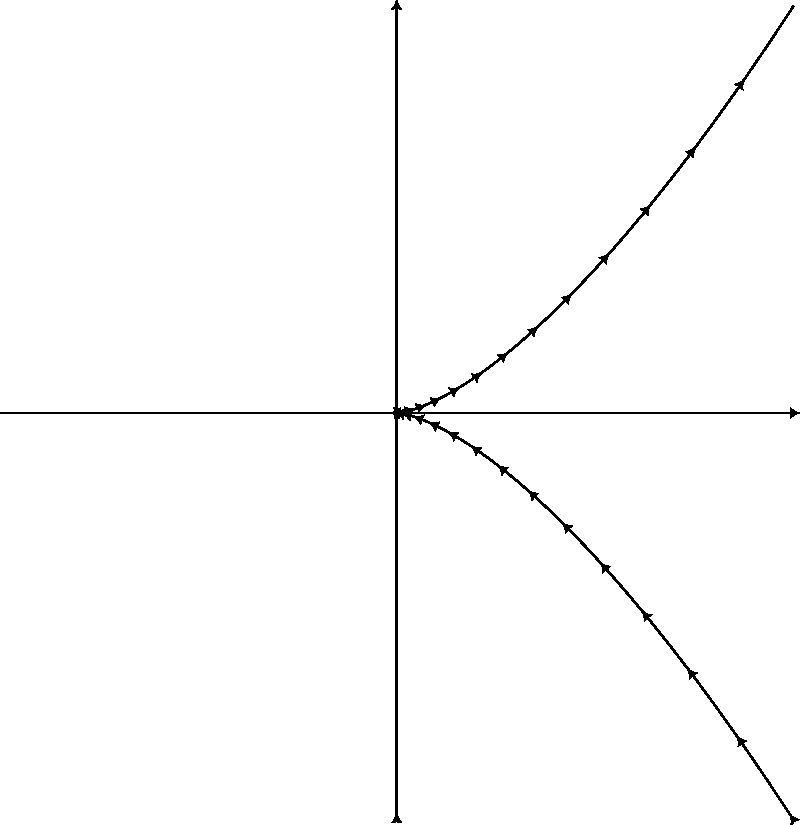
\includegraphics[width=0.5\linewidth]{semicubical_parabola.pdf}
    \end{center}

    $(0,0)$ -- точка излома (т.е. точка, в которой параметризация теряет регулярность).
\end{example}

\section{Перепараметризация}
Пусть $\phi: [a,b] \to [c,d]$, $\phi$ строго возрастает, $\phi(a) = c, \phi(b) = d$, также существует $\phi^{-1}$.
$\vf: [c,d] \to \R^3$, тогда $\vg \coloneqq \vf \circ \phi: [a,b] \to \R^3$.
В таком случае $\vg$ -- перепараметризация кривой и $\vf = \vg \circ \phi^{-1}$.

Если такая $\phi$ существует, то $\vf \sim \vg$ (эквивалентны).

Если образы $\vf(t)$ и $\vg(t)$ совпадают, кривые не самопересекаются,
а их параметризации регулярны, то существует такое $\phi$ и $\vf = \vg \circ \phi$.
\end{document}